
\chapter{CGM Statistical Modeling and Validation}
\label{sec:CGMStatisticalModelingAndValidation}

Identifiability is highly dependent on the quality of the measurements obtained. In this chapter the focus will move from the improvement of experiments towards the analysis and improvement of data acquisition devices. Sensor induced errors are one of the main problems in diabetes experimentation nowadays. Continuous glucose monitoring (CGM) devices estimate plasma glucose from interstitial glucose measurements every 1-5 minutes. They are potentially much more informative than the traditional and sparse method based on capillary self-monitoring of blood glucose. However, CGM devices are only approved as adjunctive to capillary self-monitoring due to their low accuracy.

Despite its relevance to the interpretation of glycaemic time-series and to the implementation of a future artificial pancreas, few studies have investigated the error characteristics of current CGM devices, especially in the postprandial state. Breton \textit{et al.} \cite{breton2008analysis} developed an error model for CGM based on a posteriori recalibrated data from the FreeStyle Navigator\texttrademark  (Abbott Diabetes Care, Alameda, USA). However, in contrast to real-time calibration algorithms, a posteriori recalibration implies the use of all reference BG points to minimize the sensor readings-reference glucose mismatch. In addition, Facchinetti \textit{et al.} \cite{facchinetti2010modeling} demonstrated using simulation studies how small errors in data recalibration can affect the derived statistical properties for the error. Recently, Facchinetti \textit{et al.} published a study \cite{facchinetti2013modeling} on the error of the SEVEN\textsuperscript{\textregistered} PLUS sensor (also under review in this thesis) where the diabetic subjects wore four sensors during a 9 hour study, to a total of 36 monitoring sessions. The sensors were tested against a HemoCue Glucose 201 Analyzer, using standard calibration procedures. The sensors showed clear correlations between them, and AR models were used for adjustment of the error, providing an accurate CGM error model and the factor that compose them. No simulation model of the sensor was provided, and no correlation with the blood glucose signal was provided. Therefore, error characterization of real-time CGM devices in the postprandial state is still an open issue and an area for additional investigation.

In this chapter an analysis and modeling of the postprandial error of two commercial real-time CGM devices is performed, namely the Dexcom\textsuperscript{\textregistered} SEVEN\textsuperscript{\textregistered} PLUS and the Medtronic\textsuperscript{\textregistered} Paradigm\textsuperscript{\textregistered} Veo\texttrademark{}, that were simultaneously worn by subjects with type 1 diabetes following a set of four standardized mixed meals. Statistical properties of the signal error were analyzed and a new simulation model was generated aiming for its integration into in silico studies.

\section{Data and methodology}
\label{sec:MethodologyAndData}

Twelve subjects with type 1 diabetes treated with continuous subcutaneous insulin infusion (CSII) (male/female 3/9, age $41.8�7.3$ years, diabetes duration $20�10$ years, HbA1c $8.0�0.6\%$) were studied in the postprandial state under controlled conditions, on four different occasions. Patients were monitored twice when eating a standardized meal with 40 g CHO content and twice, in addition, when they received a 100 g CHO meal. On each occasion, CGM was performed simultaneously with a SEVEN\textsuperscript{\textregistered} PLUS (Dexcom, San Diego, USA) device and a Paradigm\textsuperscript{\textregistered} Veo\texttrademark{} (Medtronic, Northridge, USA) device. 

Both devices were inserted the day before the experiment, in order to allow the devices to stabilize before the experiments. During the first day the monitors were calibrated according to the manufacturer instructions using the same capillary measurements. The day of the experiment, the devices were calibrated using the same capillary measurement obtained in fasting state.

The patients arrived at 9:00 AM to the clinic. Pre-prandial plasma glucose was standardized around 100 mg/dL by means of a feedback insulin infusion. At 13:00 h, patients ate the standardized meal and received the corresponding insulin bolus using a subcutaneous insulin infusion system. Plasma glucose levels were measured for 5 hours after the meal, every 5 minutes the first two hours after the meal and every 10 minutes afterwards, thus obtaining more frequent measurements during the meal rise phase. Plasma blood glucose levels were measured on arterialized venous blood using a reference method (YSI 2300 STAT Plus Glucose analyzer, YSI Yellow Springs, Ohio, USA), and synchronously compared with CGM's subcutaneous measurements (5 min frequency). Only forty-seven datasets were available for analysis when the SEVEN\textsuperscript{\textregistered}  PLUS device was used, because one dataset was discarded due to a flat sensor measurement at 40 mg/dL during the whole duration of the experiment. In the case of the Paradigm\textsuperscript{\textregistered} Veo\texttrademark{} device, only 42 datasets were available because the first 6 experiments were not monitored with this device. 

YSI data is assumed to be very accurate, especially if compared with any CGM device. Nowotny \textit{et al.} \cite{nowotny2012precision} evaluated the accuracy of the YSI 2300 Glucose Analyzer among other devices, showing errors of 2.2\% . This is higher than previous reference methods, and also better than the rest of the analyzers evaluated.

In order to obtain a time series of the same sample size, YSI data were linearly interpolated in the late postprandial period in order to obtain a 5 minutes periodic consistent dataset, and be able to compare it with the CGM data. Although interpolation of reference data can introduce undesired dynamics when modeling, in this case interpolation only occurs in the late postprandial period, where dynamics of both the glucose and the monitor were slower. In addition, linear interpolation were used in literature before, in the context of glucose modeling of sensor signals \cite{breton2008analysis,facchinetti2007reconstruction} where reference measurements were sparse (15 minutes). 

The signal analyzed was the CGM error calculated as:

\begin{equation}
	E(k)=CGM(k)-YSI(k)
\label{eq:cgmerror}
\end{equation}

where $E(k)$ is the error at time $k$, $CGM(k)$ is the CGM signal and $YSI(k)$ the reference blood glucose, both at the same time $k$. Some issues were taken into account in the analysis. First, the existence of a physiological delay between subcutaneous and plasma glucose, which could be patient-specific \cite{kamath2009analysis}. Second, filters included in the CGM devices may introduce additional delays (signal-processing delays). Both types of delays represent a confounder factor of CGM accuracy and should be compensated prior to further study of the error.  Third, stationarity of the error time-series should be investigated since non-stationarity may yield misleading probability distributions. Indeed, when fitting probability distribution and time-correlation of a signal, stationarity of the process is assumed. In the event of having a time varying stochastic process, non-linear transformations must be applied to the signal so that it becomes as time unvarying as possible \cite{box1994time}. The choice of the non-linear transformation to be used usually depends on the problem and the data available. 

\begin{figure}[hbtp]
\centering
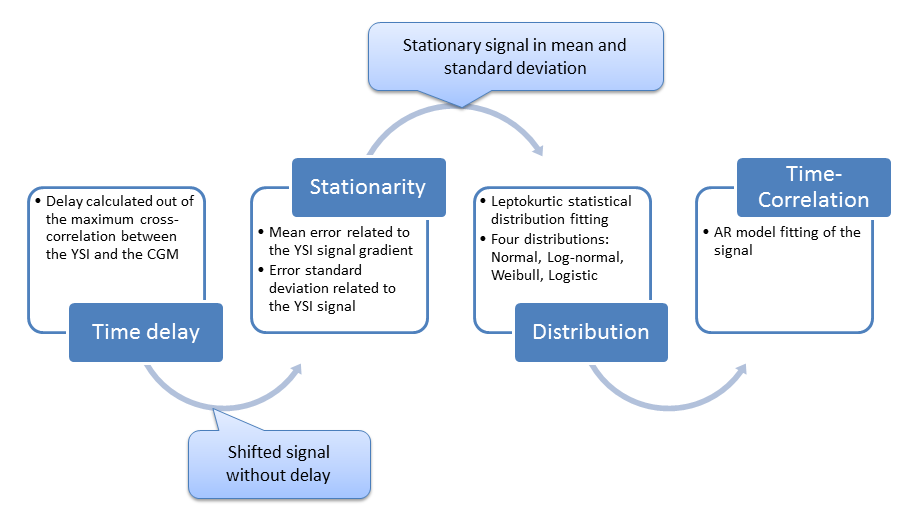
\epsfig{file=Figures/CGMmodelflow.png, width=\textwidth}\caption{Summary of stepwise statistical analysis process.}
\label{fig:CGMmodelflow}
\end{figure}

The analysis described in Figure \ref{fig:CGMmodelflow} was followed for both CGM devices:

\begin{enumerate}
	\item The delay of the CGM signal with respect to reference glucose was computed as the lag with maximum CGM versus YSI cross-correlation for each patient. A probability distribution function was fitted to the delay's histogram using a classical maximum likelihood (ML) estimator from Matlab Statistics Toolbox. Error time-series were then shifted by the corresponding delay for compensation prior to next analysis thus ``synchronizing'' CGM and reference glucose signals.
	\item Stationarity of the shifted error time-series was analyzed. A signal was considered to be stationary if time invariance of the statistical moments held. Mean and standard deviation of the error signal were calculated across the population of sensors in every instant of the postprandial period in order to obtain a time dependent signal. Time dependence of the mean and the standard deviation was analyzed. Besides graphical inspection, datasets were fitted to autoregressive (AR) models and the presence of a unit root was investigated (random walk process in the case of first order models). A stationary process should have no unit roots.
	\item Finally, the sample probability distribution for the error was analyzed and an AR model fitted to reproduce time correlation and for simulation purposes. A set of candidate probability distribution functions was defined and ML estimators in Matlab Statistics Toolbox were used for data fitting for every distribution. A simple quadratic error index was used to measure the fit for comparison purposes.
\end{enumerate}

	When performing a linear regression or just a simple correlation between variables, correlations were tested to be statistically significant using a t-statistic testing the null hypothesis of non-correlation

\section{CGM Modelling}
\label{sec:CGMModelling}

Both CGM devices were first compared to the reference measurements in order to get a general error magnitude of each error. For this comparison, the MARD (Mean Absolute Relative Deviation) was computed, following the next formula:

\begin{equation}
  MARD:= \frac{\sum_{i=1}^{n} \left| (CGM_i - YSI_i) / YSI_i \right| \cdot 100}{n}
\label{eq:mard}
\end{equation}

where $n$ is the number of samples, $CGM_i$ stands for the sensor glucose reading at time $i$ and $YSI_i$ is the reference glucose at time $i$. The SEVEN\textsuperscript{\textregistered}  PLUS monitor showed a MARD of 17.28\%, and the VEO monitor 20.12\%, for the whole dataset. 

\begin{figure}[hbtp]
\centering
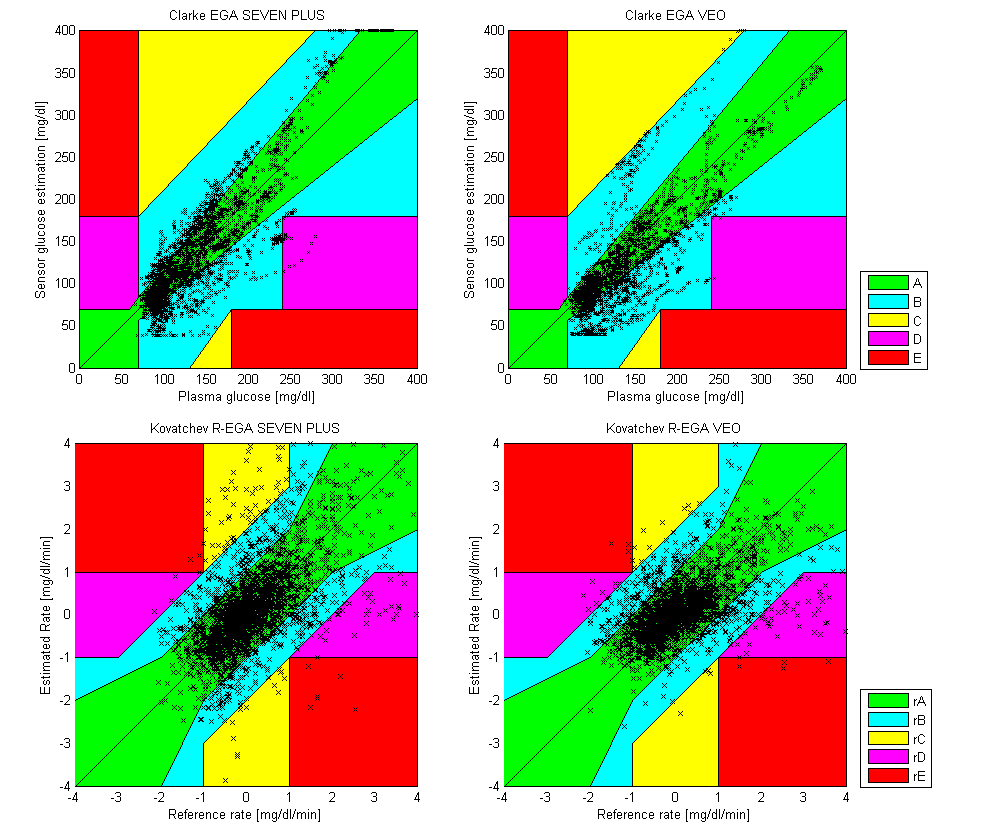
\epsfig{file=Figures/errorgrids.png, width=\textwidth}\caption{Clarke error grid (EGA) and rate error grid from continuous glucose-EGA plots for both monitors. Top row shows Clarke EGA plots, observed glucose reference measurements \textit{versus} the prediction of the monitors, SEVEN\textsuperscript{\textregistered} PLUS on the left and VEO on the right. On the bottom row, the rate error grid from continuous glucose-EGA is displayed, for the SEVEN\textsuperscript{\textregistered} PLUS on the left and VEO on the right.}
\label{fig:errorgrids}
\end{figure}

Clinical accuracy for both datasets is illustrated in Figure \ref{fig:errorgrids} using two complementary error grid analysis (EGA) methods: the Clarke-EGA \cite{clarke1987evaluating} and the glucose-rate grid proposed by Kovatchev \textit{et al.} \cite{kovatchev2004evaluating}. Regarding the Clarke grid, both monitors show very similar behavior. The SEVEN\textsuperscript{\textregistered} PLUS monitor placed 73.04\% of the data pairs in zone A, and 26.41\% in zone B, while Veo system had 66.23\% of the data pairs in zone A, and 33.25\% in zone B. Both monitors had less of 1\% of the monitoring data within the zones C, D or E. Regarding the glucose rate grid, the SEVEN\textsuperscript{\textregistered} PLUS monitor had 80.96\% of data points in zone A, 14.89\% in zone B, 2.41\% in zone C, 1.42\% in zone D and 0.32\% in zone E. Veo monitor showed 83,37\% of the data points within the zone A, 13.53\% in zone B, 0.67\% in zone C,  2.10\% in zone D, and 0.31\% in zone E.

A representative CGM trace from each device is shown in Figure \ref{fig:CGMsamples}. The YSI signals shown correspond to different patients following the detailed experiments. In the SEVEN\textsuperscript{\textregistered} PLUS monitor sample, a rapidly increasing glucose concentration after the meal is observed, followed by a slow decreasing glucose in the late postprandial period. The VEO monitor sample shows a rapidly increasing glucose response right after the meal and a rebound increase in the late postprandial period. It can be appreciated that both monitors have trends similar to the YSI signal they are estimating.

\begin{figure}[hbtp]
\centering
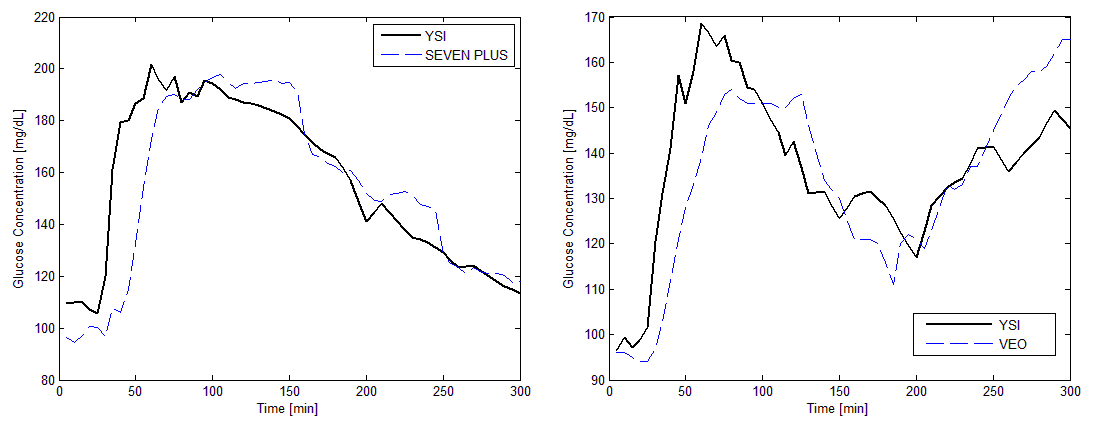
\epsfig{file=Figures/CGMsamples.png, width=\textwidth}\caption{Representative sample of two different postprandial periods for the two monitors. The left panel shows the SEVEN\textsuperscript{\textregistered} PLUS monitor sample and the right panel shows the VEO monitor sample.}
\label{fig:CGMsamples}
\end{figure}

\subsection{Analysis of delay}
\label{sec:AnalysisOfDelay}

The delay histogram for all the available datasets is shown in Figure \ref{fig:delaymodelfit}. This delay was consistent throughout the entire postprandial period, and no significant difference on the calculated delays was achieved by considering only the first two hours (transient) of the entire postprandial period. Observing the time correlation of the datasets, in the SEVEN\textsuperscript{\textregistered} PLUS monitor, 28 showed no significant delay between the two signals (i.e, delay was less than five minutes due to the CGM resolution), and 19 for the Paradigm\textsuperscript{\textregistered} Veo\texttrademark{} .

\begin{figure}[hbtp]
\centering
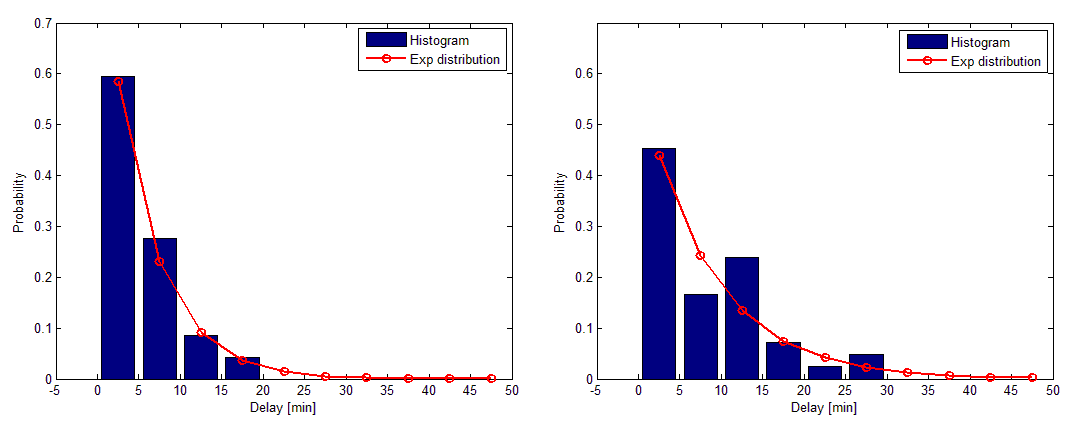
\epsfig{file=Figures/delaymodelfit.png, width=\textwidth}\caption{Delay-time histograms for the SEVEN\textsuperscript{\textregistered} PLUS monitor (left) and the Paradigm\textsuperscript{\textregistered} Veo\texttrademark{} (right).}
\label{fig:delaymodelfit}
\end{figure}

The histogram analysis hinted that the delay follows an exponential probability distribution:
\begin{equation}
  f(x)=\frac{1}{\mu} e^{-\frac{x}{\mu}}
\label{eq:exponential}
\end{equation}

where $\mu$ is the exponential parameter. The exponential parameter was adjusted for each monitor. For the SEVEN\textsuperscript{\textregistered} PLUS monitor the parameter was $\tau_{sevenplus}=1.08$ with a 95\% confidence interval $[0.82,1.46]$ and for the Paradigm\textsuperscript{\textregistered} Veo\texttrademark{} $\tau_{veo}=1.69$ with a 95\% confidence interval $[1.28,2.35]$, resulting in the curve fitting shown in red in Figure \ref{fig:delaymodelfit}.

The observed delay for the SEVEN\textsuperscript{\textregistered} PLUS device was consistent with previous works \cite{zisser2009accuracy} for the SEVEN\textsuperscript{\textregistered} system, where an average value of 5 minutes is reported as the lag for maximum cross-correlation. However, no probability distribution for the delay was reported for comparison. Compared with the Dexcom system, the Paradigm\textsuperscript{\textregistered} Veo\texttrademark{} showed a significant (p=0.007) larger average delay (8 minutes). Our results were slightly larger than those reported by Keenan \textit{et al.} \cite{keenan2010accuracy}, but neither these values nor the SEVEN\textsuperscript{\textregistered} Plus values were comparable due to the difference in computation methods. Therefore, measurement of the delay should be standardized in order to enable comparisons between different studies. Additionally, the Paradigm\textsuperscript{\textregistered} Veo\texttrademark{} exhibited a slower decay in the fitted exponential distribution, indicating higher variability of the delay value up to 30 minutes. 

\subsection{Analysis of Stationarity}
\label{sec:AnalysisOfStationarity}

The statistical moments of the data analyzed after delay compensation were not time invariant, as shown in Figure \ref{fig:stationarityexperimental}. For both monitors, the mean and standard deviation of the error were non-stationary. Our goal was to find a transformation of the signal in order to make it as close to stationary as possible. This transformation had to be invertible for simulation purposes. This means that the transformation had to be based on available information in the simulation context, e.g., plasma glucose from a glucoregulatory model, or equivalently, the YSI signal from the experimental data.

\begin{figure}[hbt]
\centering
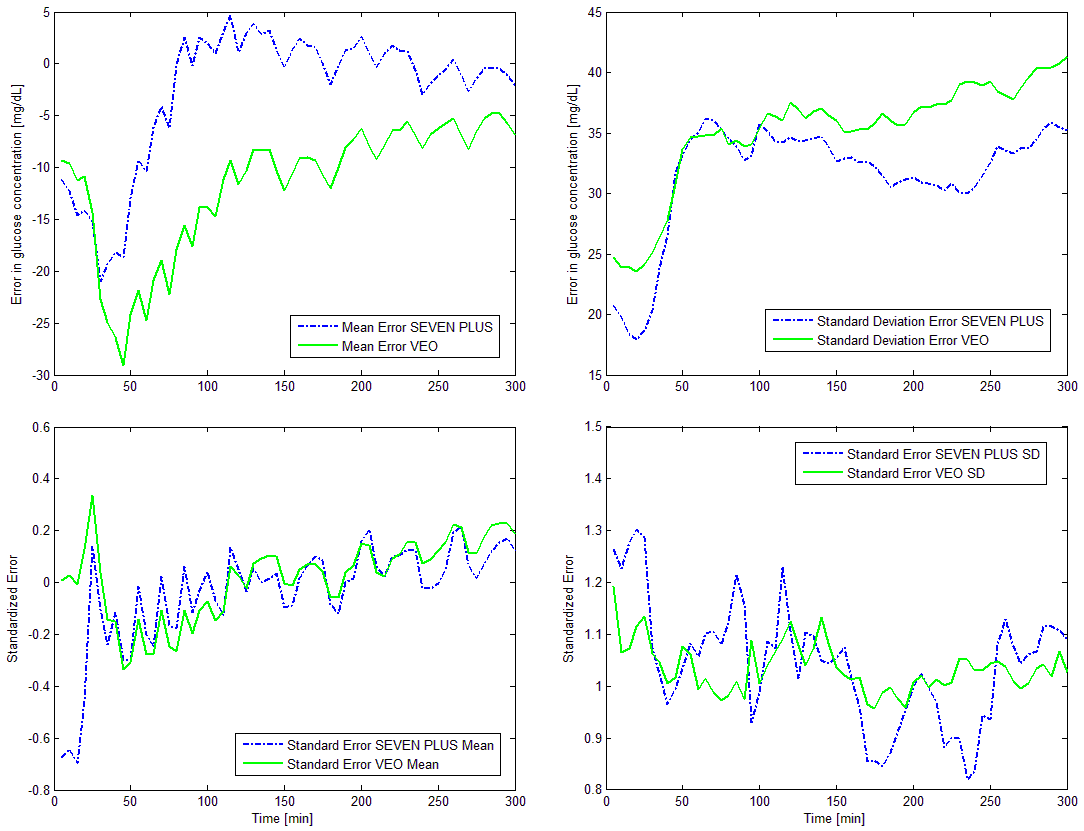
\epsfig{file=Figures/stationarityexperimental.png, width=\textwidth}\caption{Top panels show the meal error and standard deviation of the error after delay compensation for the SEVEN\textsuperscript{\textregistered} PLUS and the Paradigm\textsuperscript{\textregistered} Veo\texttrademark{} monitors. Bottom panels show the same signals after the standardization process. The left figures show the mean error for both monitors while on the right the standard deviation of the error signals is represented. Notice the different scales on all four plots.}
\label{fig:stationarityexperimental}
\end{figure}

In general, stationarity of the error time-series is assumed when fitting probability distributions to a stochastic signal. However, it can be observed that these assumptions were not correct when interpreting the error of CGM in the postprandial state. Mean and standard deviation after delay compensation were both time-varying, especially for the first two hours after a meal intake. This may be related to the performance of the real-time calibration algorithm after the high rise of glucose following the intake up to its peak value.

Despite the standardization of the initial conditions by means of an insulin feedback phase, both monitors had an initial mean underestimation of glucose of 10 mg/dL. Surprisingly this value was equal to both devices. It is unknown to the author whether it may correspond to a setting of the manufacturers. An initial standard deviation of 20-25 mg/dL was observed yielding significant errors. 

Both monitors were worn simultaneously by the patient and calibrated with the same calibration points obtained in fasting state the same day of the experiment. Calibration points have been recognized as crucial factors influencing the accuracy of CGM readings \cite{buckingham2006,wolpert2008}. In this case, the calibration performed was done 4-5 hours before the experiment in fasting state, and it did not seem to induce differences between both devices.

After meal intake, both devices were unable to follow the high rise of glucose, increasing the initial underestimation up to a peak value (approximately 20 mg/dL for SEVEN\textsuperscript{\textregistered} Plus and 30 mg/dL for the Paradigm\textsuperscript{\textregistered} Veo\texttrademark{}) about 50 minutes later. The particular sensor delay should be additionally considered for a correct interpretation. During this time, the error standard deviation increased steadily, having a similar peak time as the mean error, with a peak value of 35 mg/dL for both monitors. 

After this initial period, the glucose underestimation decreased. The CGM glucose estimation recovered slowly towards the glucose reference value. A faster recovery was observed by the SEVEN\textsuperscript{\textregistered} PLUS. It is noteworthy that approximately zero mean error was observed for the SEVEN\textsuperscript{\textregistered} PLUS monitor after peak time, in contrast to VEO signal, which appears to be showing a bias in the mean error. This bias converged slowly to zero, but the 5 hours postprandial monitoring window we used here was insufficient for capturing the whole stabilization of the mean error in the VEO monitor.

If variability of CGM readings were reduced, our results suggest that CGM would allow for a good representation of postprandial glucose. Regarding the standard deviation, a plateau at 35 mg/dL was reached for the SEVEN\textsuperscript{\textregistered} PLUS, while a slight increasing trend was obtained for the Paradigm\textsuperscript{\textregistered} Veo\texttrademark{}. Thus, the meal event represented a big challenge for both devices producing a significant variability, which is still a major issue in CGM performance. Certainly, sources of this variability should be investigated in future studies to confirm whether it is due to variability of the physiological delay, the intensity signal produced by the sensor or the calibration algorithm itself. 

A positive correlation between the YSI signal and the standard deviation of the error was found. This is an indication of the variability of the sensor to capture the postprandial peak. In addition, a negative correlation of the YSI rate of change and the mean of the error reflects that sensor readings were falling behind the reference glucose in the rising trend (the error becomes more negative in average), in spite of delay compensation. 

The second moment of the error signal closely resembled the YSI blood glucose measurements for both monitoring systems. The correlation coefficient for the SEVEN\textsuperscript{\textregistered} PLUS monitor was $r_{sevenplus}=0.93$ ($range_{95\%} = [0.90, 0.96]$) and for the Paradigm\textsuperscript{\textregistered} Veo\texttrademark{} $r_{veo}=0.82$ ($range_{95\%} = [0.72, 0.89]$), both significant ($p<0.005$). The regression lines for these correlations were:
\begin{align}
	\text{SEVEN PLUS: }STD(k) &=0.3142 \cdot YSI(k)-12.9056 \label{eq:std_corr1} \\
	\text{VEO: }STD(k) &=0.2711 \cdot YSI(k)-3.7679 \label{eq:std_corr2}
\end{align}

where $STD(k)$ is the standard deviation of the error at time $k$. 

As for the mean of the error signal, the correlation with the raw YSI signal did not show a significant correlation coefficient. The correlation with the gradient of the YSI signal was better, with a coefficient of $r_{sevenplus}=-0.79$ ($range_{95\%} = [-0.87, -0.68]$) and $r_{veo}=-0.54$ ($range_{95\%} = [-0.70, -0.33]$), both being statistically significant ($p<0.005$). This correlation was not as evident as the one with the second moment, but it was much better than the correlation found to any other signal derived from the YSI. Regarding to the correlations found we can guess that stationarity achieved with these transformations was better in the SEVEN\textsuperscript{\textregistered} PLUS monitor than in the Paradigm\textsuperscript{\textregistered} Veo\texttrademark{}. The regression line for the correlation of the first moment was:
\begin{align}
	\text{SEVEN PLUS: } & Mean(k)=-2.0046\cdot dYSI(k)/dt-1.0628 \label{eq:mean_corr1} \\ 
	\text{VEO: } & Mean(k)=-1.323\cdot dYSI(k)/dt-10.517 \label{eq:mean_corr2}
\end{align}

where $Mean(k)$ is the average error at time $k$.
Again, as it happened with the delays, these regressions were consistent throughout the entire postprandial period. Considering these regressions as good characterizations of the statistical moments of the signals, the error signal can be transformed as follows, so that it becomes (quasi-)stationary: 

\begin{equation}
	\bar{E}(k)=\frac{E(k)-Mean(k)}{STD(k)}
\label{eq:error_standard}
\end{equation}

In case of perfect estimation of the mean and standard deviation at time $k$, the transformed error signal $\bar{E}(k)$ will have zero mean and unity standard deviation throughout the postprandial period.

Stationarity of the signal was improved after this transformation, as shown by the roots of the AR models fitted before and after the ``standardization''. The error signals were tested to fit AR models, looking for the lowest-order model with random uncorrelated residuals. The transformed statistical moments along time can also be seen in Figure \ref{fig:stationarityexperimental}, where a clear improvement on stationarity of both signals can be appreciated comparing top and bottom panels.

The SEVEN\textsuperscript{\textregistered} PLUS time-series showed a good fitting to a first order AR model before and after the transformation. The model root was $z=0.9892$ before the transformation, and $z=0.9249$ after. The transformation moves the dynamics of the data away from those of a random walk (unit root), thus making it more stationary.
The Paradigm\textsuperscript{\textregistered} Veo\texttrademark{} time-series adjusted well to a first order AR model before the transformation and to a third order model after. The model root before the transformation was $z=0.9977$, reaffirming the non-stationarity of the process. After the transformation, the model root closer to unity was $z=0.9846$, showing some improvement towards stationarity, but not as much as in the SEVEN\textsuperscript{\textregistered} PLUS. Correlations were weaker in the case of the Paradigm\textsuperscript{\textregistered} Veo\texttrademark{} which translated into a worse compensation for non-stationarity.

\subsection{Distribution fitting}
\label{sec:DistributionFitting}

The datasets used for distribution and auto-correlation fitting were already transformed following the delay compensation and the standardization processes explained before. Kurtosis was high for both datasets, so leptokurtic distributions were used for fitting. Asymmetry was very low in the data, but some non-symmetric distributions were also tested. Four different statistical distributions were finally considered:
\begin{align}
	\text{Weibull: }  f(x) & =\frac{k}{\lambda}\left( \frac{x}{\lambda}\right)^{k-1} e^{-\left(x/\lambda \right)^k} \label{eq:distributions1} \\  
	\text{Normal: } f(x) &=\frac{1}{\sqrt{2 \pi \sigma^2}} e^{-(x-\mu)^2 /2 \sigma^2} \label{eq:distributions2} \\ 
	\text{Log-Normal: }  f(x) &=\frac{1}{x \sigma \sqrt{2 \pi \sigma^2}} e^{-(log x - \mu)^2 /2 \sigma^2} \label{eq:distributions3} \\ 
	\text{Logistic: } f(x) &=\frac{1}{1+e^{\frac{x-\mu}{s}}}  \label{eq:distributions4}
\end{align}

Five Paradigm\textsuperscript{\textregistered} Veo\texttrademark{} sensors showed unusual behaviors with very big mean absolute errors (over 50 mg/dL), even though their calibrations were correct. These offsets produced a multimodal histogram (see Figure \ref{fig:distributionfit}). Given that this behavior was only observed in 5 sensors, those monitoring periods were not used to fit a probability distribution, remaining a total of 37 datasets. Given that the SEVEN\textsuperscript{\textregistered} PLUS did not register faulty monitoring periods, the Paradigm\textsuperscript{\textregistered} Veo\texttrademark{} seems to be more prone to abnormal sensor behaviors. This should be confirmed with larger studies.


\begin{figure}[hbtp]
\centering
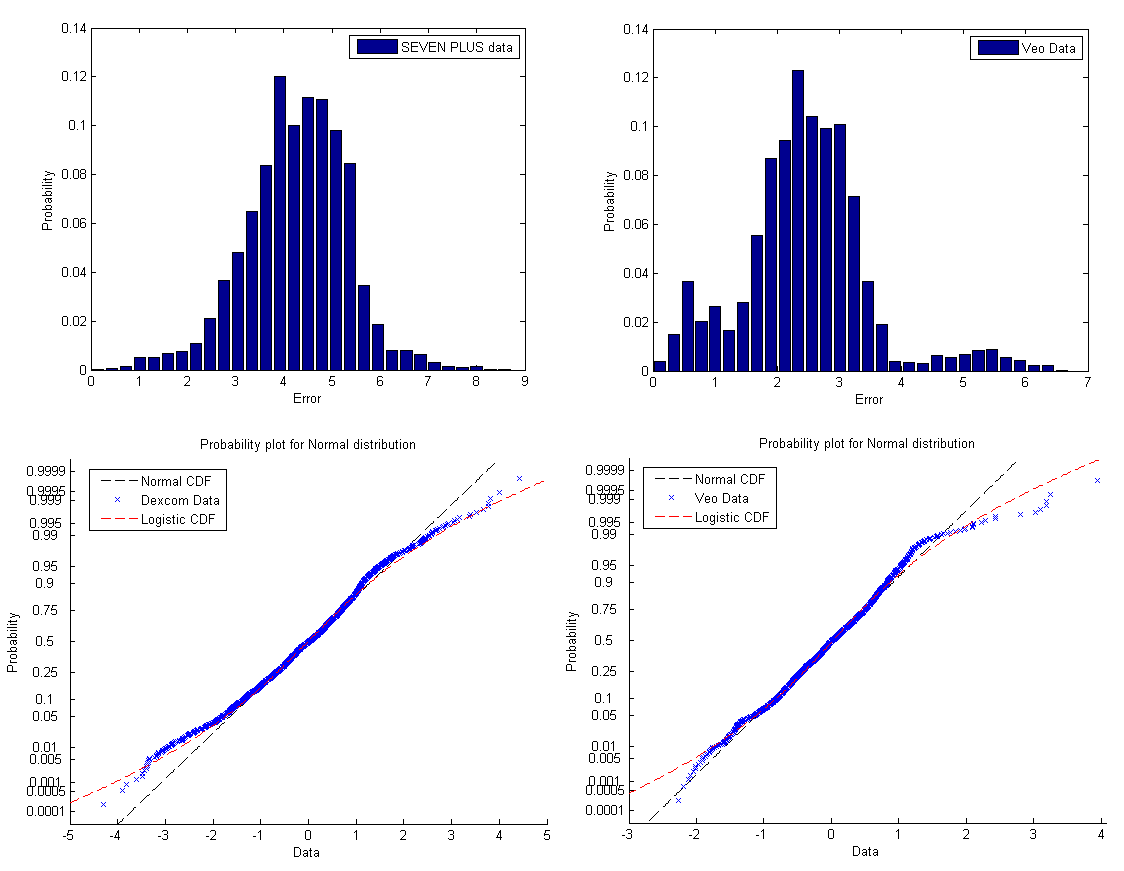
\epsfig{file=Figures/distributionfit.png, width=\textwidth}\caption{Histograms of the standardized error (top) and scaled cumulative distribution (bottom) plots for the SEVEN\textsuperscript{\textregistered} PLUS monitor (left) and the Paradigm\textsuperscript{\textregistered} Veo\texttrademark{} (right).}
\label{fig:distributionfit}
\end{figure}

The Log-Normal and Weibull distributions are only defined for positive values. To cope with this problem, data were transformed by adding its absolute minimum value (equal to 4.3069 for the SEVEN\textsuperscript{\textregistered} PLUS and 2.4439 for the Paradigm\textsuperscript{\textregistered} Veo\texttrademark{}), thus making all errors positive and not centered in zero.
The estimates are shown in Table \ref{tab:distrasults}. The best estimator was given at the normal distribution for the Paradigm\textsuperscript{\textregistered} Veo\texttrademark{} ($\mu_{VEO}=2.435$ and $s_{veo}=0.5415$) and the logistic distribution for the SEVEN\textsuperscript{\textregistered} PLUS ($\mu_{sevenplus}=4.297$ and $s_{sevenplus}=0.587$). Probability plots for the logistic and normal distribution are shown in Figure \ref{fig:distributionfit}. However, the difference between the fit of the logistic distribution and the normal distribution for the SEVEN\textsuperscript{\textregistered} PLUS was almost negligible ($1.92�10^{-3}$ vs $2.02�10^{-3}$). Normality assumption after all the transformations seems thus sensible.

\begin{table}[hbtp]
	\centering
	\begin{tabular}{ c | c | c | c | c | c | c }
	\hline 
	\multirow{2}{*}{Distribution} & \multicolumn{2}{c}{Parameters} & \multirow{2}{*}{Fit$\times 10^{-3}$} & \multicolumn{2}{c}{Parameters} & \multirow{2}{*}{Fit$\times 10^{-3}$} \\
   & \multicolumn{2}{c}{SEVEN\textsuperscript{\textregistered} PLUS} &  & \multicolumn{2}{c}{Paradigm\textsuperscript{\textregistered} Veo\texttrademark{}} & \\
	\hline 
	\multirow{2}{*}{Normal} & $\mu$ & $\sigma$ & \multirow{2}{*}{2.02} & $\mu$ & $\sigma$ & \multirow{2}{*}{1.39} \\
	& 4.27 & 1.057 & & 2.282 & 0.693 & \\
	\hline 
  \multirow{2}{*}{Weibull} & $a$ & $b$ & \multirow{2}{*}{2.49} & $a$ & $b$ & \multirow{2}{*}{2.56} \\
	& 4.652 & 4.329 & & 2.515 & 3.412 & \\
	\hline 
	\multirow{2}{*}{Logistic} & $\mu$ & $s$ & \multirow{2}{*}{1.92} & $\mu$ & $s$ & \multirow{2}{*}{1.84} \\
	& 4.297 & 0.587 & & 2.289 & 0.387 & \\
	\hline 
	\multirow{2}{*}{Log-normal} & $\mu$ & $\sigma$ & \multirow{2}{*}{42.6} & $\mu$ & $\sigma$ & \multirow{2}{*}{42.61} \\
	& 1.402 & 0.764 & & 0.751 & 0.866 & \\
	\hline 
	\end{tabular}
\caption{Parameters of the distribution fitting results for the SEVEN\textsuperscript{\textregistered} PLUS and the Paradigm\textsuperscript{\textregistered} Veo\texttrademark{} monitors.}
\label{tab:distrasults}
\end{table}

Finally, a first order AR model explains appropriately the error data for the SEVEN\textsuperscript{\textregistered} PLUS, which is consistent with Breton \textit{et al.} \cite{breton2008analysis}. However, a third order AR model was needed for the Paradigm\textsuperscript{\textregistered} Veo\texttrademark{}. This may be due to distinct filtering algorithms for the raw signal since both monitors use linear regression based calibration algorithms. Based on the previous analysis a model for each monitor was derived. This model incorporated time-varying statistical characteristics of the error for their integration into in silico tests for controller validations. These models are detailed in the next chapter, along with the full CGM simulation model of each monitor.

\section{Validation}
\label{sec:Validation}

Following the error signal analysis, simulation models were built for the SEVEN\textsuperscript{\textregistered} PLUS and Paradigm\textsuperscript{\textregistered} Veo\texttrademark{}   consisting on the following steps:

\begin{enumerate}
	\item A time series was generated from the fitted AR model.
	\item Transformations applied to get (quasi-)stationarity were inversely applied reproducing time varying characteristics of error mean and variance.
	\item A realization for the delay following the identified probability distribution was computed and applied.
\end{enumerate}

The SEVEN\textsuperscript{\textregistered} PLUS transformed error time-series followed a first order AR model
\begin{equation}
\bar{E}(k) = \alpha_1 \cdot \bar{E}(k-1) + \beta \cdot w(k), \,\,\,\, \bar{E}(0)=w(0)
\label{eq:AR_sevenplus}
\end{equation}
where $\bar{E}(k)$ is the correlated standardized error (output of the AR system), $w(k)$ is a white noise signal, $\alpha_1=0.9249$  is the AR parameter, and $\beta=0.3756$  is the correction of the variance factor, chosen in order to get the desired characteristics of the normal distribution for the data after filtering.  
The Paradigm\textsuperscript{\textregistered} Veo\texttrademark{} time-series followed a third-order model:
\begin{gather}
\bar{E}(k)=\alpha_1 \cdot \bar{E}(k-1)+\alpha_2 \cdot \bar{E}(k-2) +\alpha_3 \cdot \bar{E}(k-3)+\beta \cdot w(k) \nonumber \\
\bar{E}(0)= w(0), \,\,\,\, \bar{E}(1)=w(1) \label{eq:AR3_veo}
\end{gather}
with : $\alpha_1=0.9471$, $\alpha_2=-0.1936$, $\alpha_3=0.2271$ and $\beta=0.2198$.

The white noise used as input of the AR models follows the normal distribution fitted to the data in the previous chapter. Normality was assumed for both monitors. For the SEVEN\textsuperscript{\textregistered} PLUS the mean was $\mu_{SEVENPLUS}=4.27$ and the standard deviation $\sigma_{SEVENPLUS}=1.057$, considering a shift of 4.3069. For the Paradigm\textsuperscript{\textregistered} Veo\texttrademark{} the parameters were: $\mu_{Veo}=2.282$ $\sigma_{Veo}=0.693$, and a shift of 2.4439.

In order to reproduce the time-variance of the error mean and standard deviation, we had to invert the standardization applied to the CGM error data during the analysis process, i.e.:
\begin{equation}
E(k)=STD(k) \cdot \bar{E}(k)+Mean(k)
\label{eq:standardization_invert}
\end{equation}

$STD(k)$ and $Mean(k)$ were calculated as: 
\begin{align} 
	\text{SEVEN PLUS: } STD(k) &=0.3142 \cdot \widetilde{PG}(k)-12.9056               \label{eq:standardization1} \\
	\text{VEO: } STD(k) & =0.2711 \cdot \widetilde{PG}(k)-3.7679                      \label{eq:standardization2} \\
	\text{SEVEN PLUS: } Mean(k) &=-2.0046 \cdot \frac{d\widetilde{PG}(k)}{dt}-1.0628  \label{eq:standardization3} \\
	\text{VEO: } Mean(k) &=-1.323 \cdot \frac{d\widetilde{PG}(k)}{dt}-10.517          \label{eq:standardization4}
\end{align}

where $\widetilde{PG} (k)$ is the plasma glucose given by the virtual patient simulator, or in case of using real patient data, the plasma glucose measurements. The CGM readings were then calculated by adding the error to the simulator glucose output, and shifting $d$ steps, where $d$ is a realization of an exponential distribution $Exp(\mu)$:
\begin{gather}
CGM(k)= \widetilde{PG}(k-d)+E(k-d), \,\, d=Exp(\mu) \nonumber \\
\mu_{sevenplus}=1.08, \,\, \mu_{veo}=1.69 \label{eq:exp_realization}
\end{gather}

An illustration of several simulation runs for both models is shown in Figure \ref{fig:simulatedCGMsamples}. Average MARD for the simulated SEVEN\textsuperscript{\textregistered} PLUS was 18.72\%, and for the simulated Paradigm\textsuperscript{\textregistered} Veo\texttrademark{} was 18.38\%. 

\begin{figure}[hbtp]
\centering
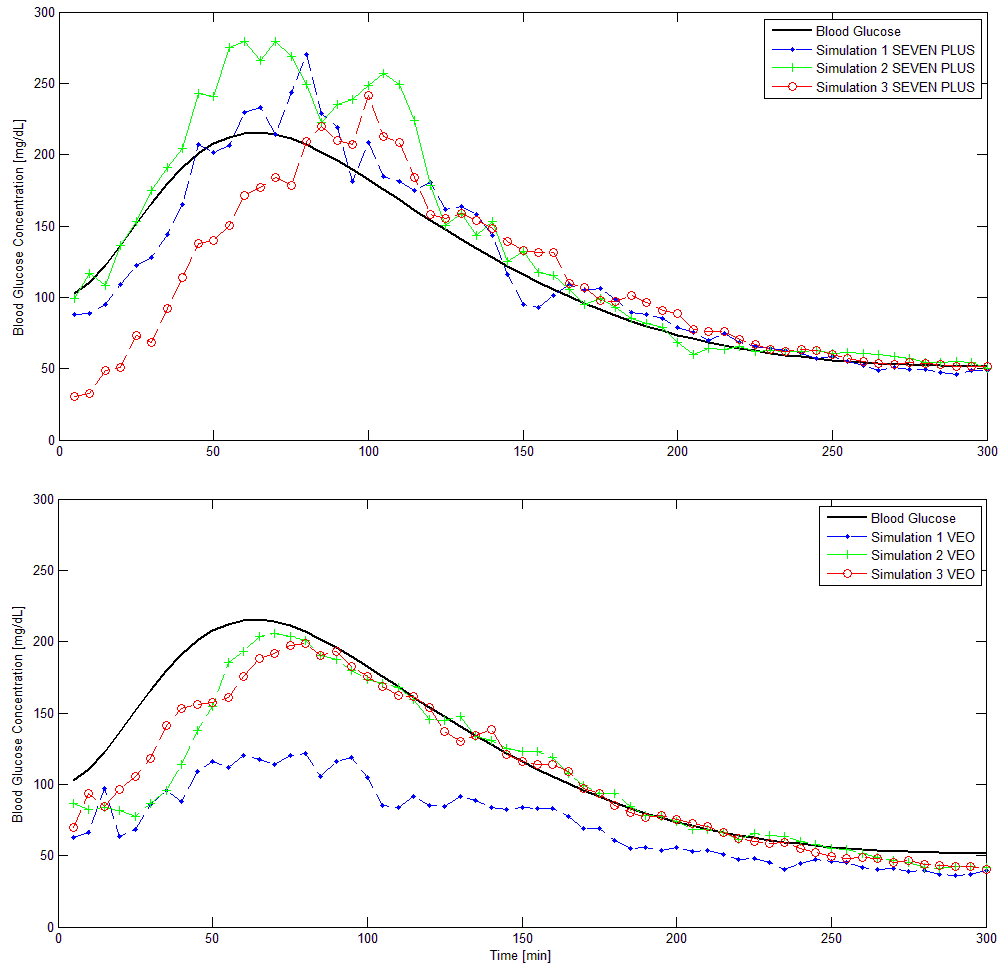
\epsfig{file=Figures/simulatedCGMsamples.png, width=\textwidth}\caption{Three simulation of each monitor with the proposed models for the postprandial period of a virtual diabetic patient. Top panel shows the SEVEN\textsuperscript{\textregistered} PLUS response while bottom panel corresponds to the Paradigm\textsuperscript{\textregistered} Veo\texttrademark{} simulations.}
\label{fig:simulatedCGMsamples}
\end{figure}

For validation purposes a virtual dataset a hundred times larger than the original dataset was created (the model was run a hundred times for each YSI trace), to better simulate the fitted distributions in their entire domain. The YSI samples used for the calculation non-stationarity of the error were extracted from the same dataset used for the model fitting. For this validation, the Paradigm\textsuperscript{\textregistered} Veo\texttrademark{} data used for comparison only comprehends predictions from the 37 sensors than showed no unusual behavior. In Figure \ref{fig:delayvalidation} validation of the signal delay is shown, comparing the probability distribution of the real dataset versus the simulated data. Figure \ref{fig:simulatedstationarity} shows the comparison of the statistical properties of the data and the simulation, as well as illustrates the time variation of the simulated data.

\begin{figure}[hbtp]
\centering
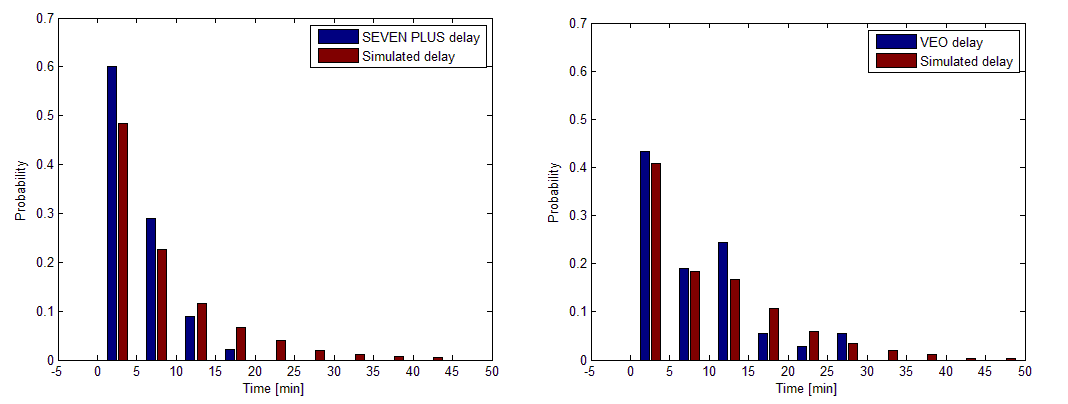
\epsfig{file=Figures/delayvalidation.png, width=\textwidth}\caption{Real and simulated delay distribution for both monitors. The left panel shows the delay of the SEVEN\textsuperscript{\textregistered} PLUS monitor, against the simulation distribution using the proposed model. In the right panel the distributions for the Paradigm\textsuperscript{\textregistered} Veo\texttrademark{} is shown.}
\label{fig:delayvalidation}
\end{figure}

Computer simulations of the adjusted model for both monitors show very similar delay distribution as the original data, as shown in Figure 8. The histograms of both simulated models are much more uniform than the original data, following closely the original exponential distribution that generated them.

\begin{figure}[hbt]
\centering
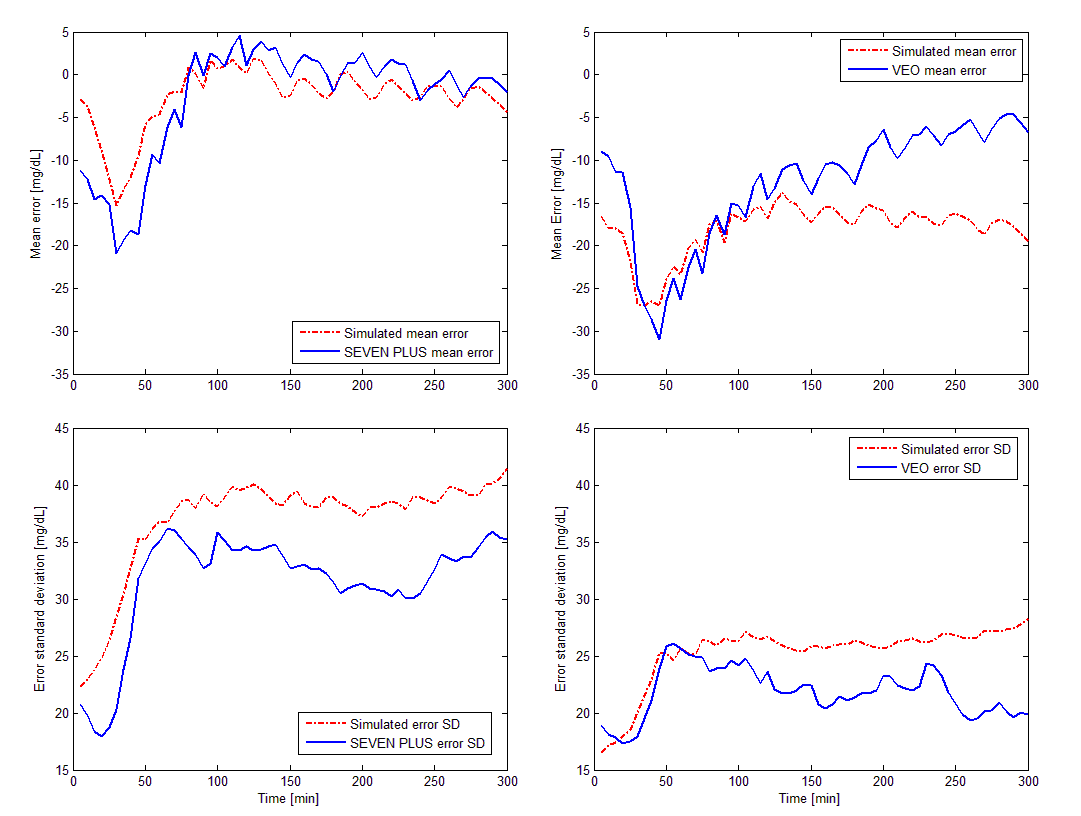
\epsfig{file=Figures/simulatedstationarity.png, width=\textwidth}\caption{Top row shows time variation of the mean error for both monitors and for the simulated error. In the bottom row the standard deviation of the error and the simulation is plotted against time. Left column shows the SEVEN\textsuperscript{\textregistered} PLUS data and model, and the right column illustrates the statistical behavior of the Paradigm\textsuperscript{\textregistered} Veo\texttrademark{} and its representing model.}
\label{fig:simulatedstationarity}
\end{figure}

Validation of the statistical moments and non-stationarity of the error can be extracted from Figure \ref{fig:simulatedstationarity}. Time variant mean and standard deviation were obtained for the simulated data, with similar dynamics than the original data. Mean signal was almost identical for the SEVEN\textsuperscript{\textregistered} PLUS device, but it showed an offset for the late postprandial period in the Paradigm\textsuperscript{\textregistered} Veo\texttrademark{} simulation (approx. 15 mg/dL). This was expected since the correlations for the Medtronic monitor were much lower than those of the Dexcom device. Standard deviation time variation was also very similar to that of the original error, presenting small offsets at the end of the postprandial period (approx. 5 mg/dL for the SEVEN\textsuperscript{\textregistered} PLUS and 7 mg/dL for the Paradigm\textsuperscript{\textregistered} Veo\texttrademark{}). These offsets did not contribute negatively on the clinical accuracy of the simulated error, since the overall MARD was similar for the simulated dataset and the real data, especially for the SEVEN\textsuperscript{\textregistered} PLUS. Indeed, simulated MARD for the Dexcom monitor was 18.72\%, compared to the 17.28\% of the real monitor. For the Paradigm\textsuperscript{\textregistered} Veo\texttrademark{} the simulated MARD was 18.38\%, being somewhat higher than the observed error from only 37 sensors, which was 14.98\%.

In conclusion, both models were successfully validated reproducing the same statistical properties than the original data. Importantly, although the models have been tested only against postprandial data, additional inconveniences are not expected when analyzing data in the fasting state since postprandial control is considered by far the major challenge in developing the artificial pancreas. Meal intake was a big challenge for both devices, which were unable to follow the high rise of glucose. The high observed variability in both cases threatened postprandial performance. Compared to the SEVEN\textsuperscript{\textregistered} PLUS device, the Paradigm\textsuperscript{\textregistered} Veo\texttrademark{} device seemed to exhibit longer delays and higher probability of abnormal sensor behaviors in postprandial conditions. Certainly, further improvements in calibration algorithms are needed to reduce variability in CGM. 
